\bigskip
\begin{center}
\textbf{\Large \color{red}This tutorial is currently under construction.}
\end{center}
\bigskip

\section{Overview: Gene tree-species tree models}

Ever since \cite{Zuckerkandl1965a}, researchers have acknowledged that phylogenies reconstructed from homologous gene sequences could differ from species phylogenies.
As molecular sequences accumulated, the link between gene trees and species trees started to be modeled. 
The first models were based on parsimony, and aimed for instance at reconciling a gene tree with a species tree by minimizing the number of events of gene duplication and gene loss. 
In the past dozen years, probabilistic models have been proposed to reconstruct gene trees and species trees in a rigorous statistical framework.
Models and algorithms have quickly grown in complexity, to model biological processes with increasing realism, to accommodate several processes at the same time, or to handle genome-scale data sets.
In this overview we will not detail these models, and we invite the interested reader to take a look at recent reviews (\EG \citep{Szollosi28072014}).

\subsection{Processes of discord}
There are several reasons why a gene tree may differ from a species tree. 
Of course, a gene tree may differ from the species tree just because a mistake was made during the analysis of the gene sequences, at any point in a pipeline going from the sequencing itself to the tree reconstruction.
Such a mistake would produce an incorrect gene tree.
Here we do not mean this kind of discord, but rather discord that comes from a real biological process that generates true gene histories that differ from true species histories.
These processes include gene duplication, gene loss, gene transfer (used loosely here to also include reticulation, hybridization between species), and incomplete lineage sorting (Fig. \ref{fig1}). 
Incomplete lineage sorting will be discussed in more details in the following subsection.

\begin{figure}[h!]
\centering
\fbox{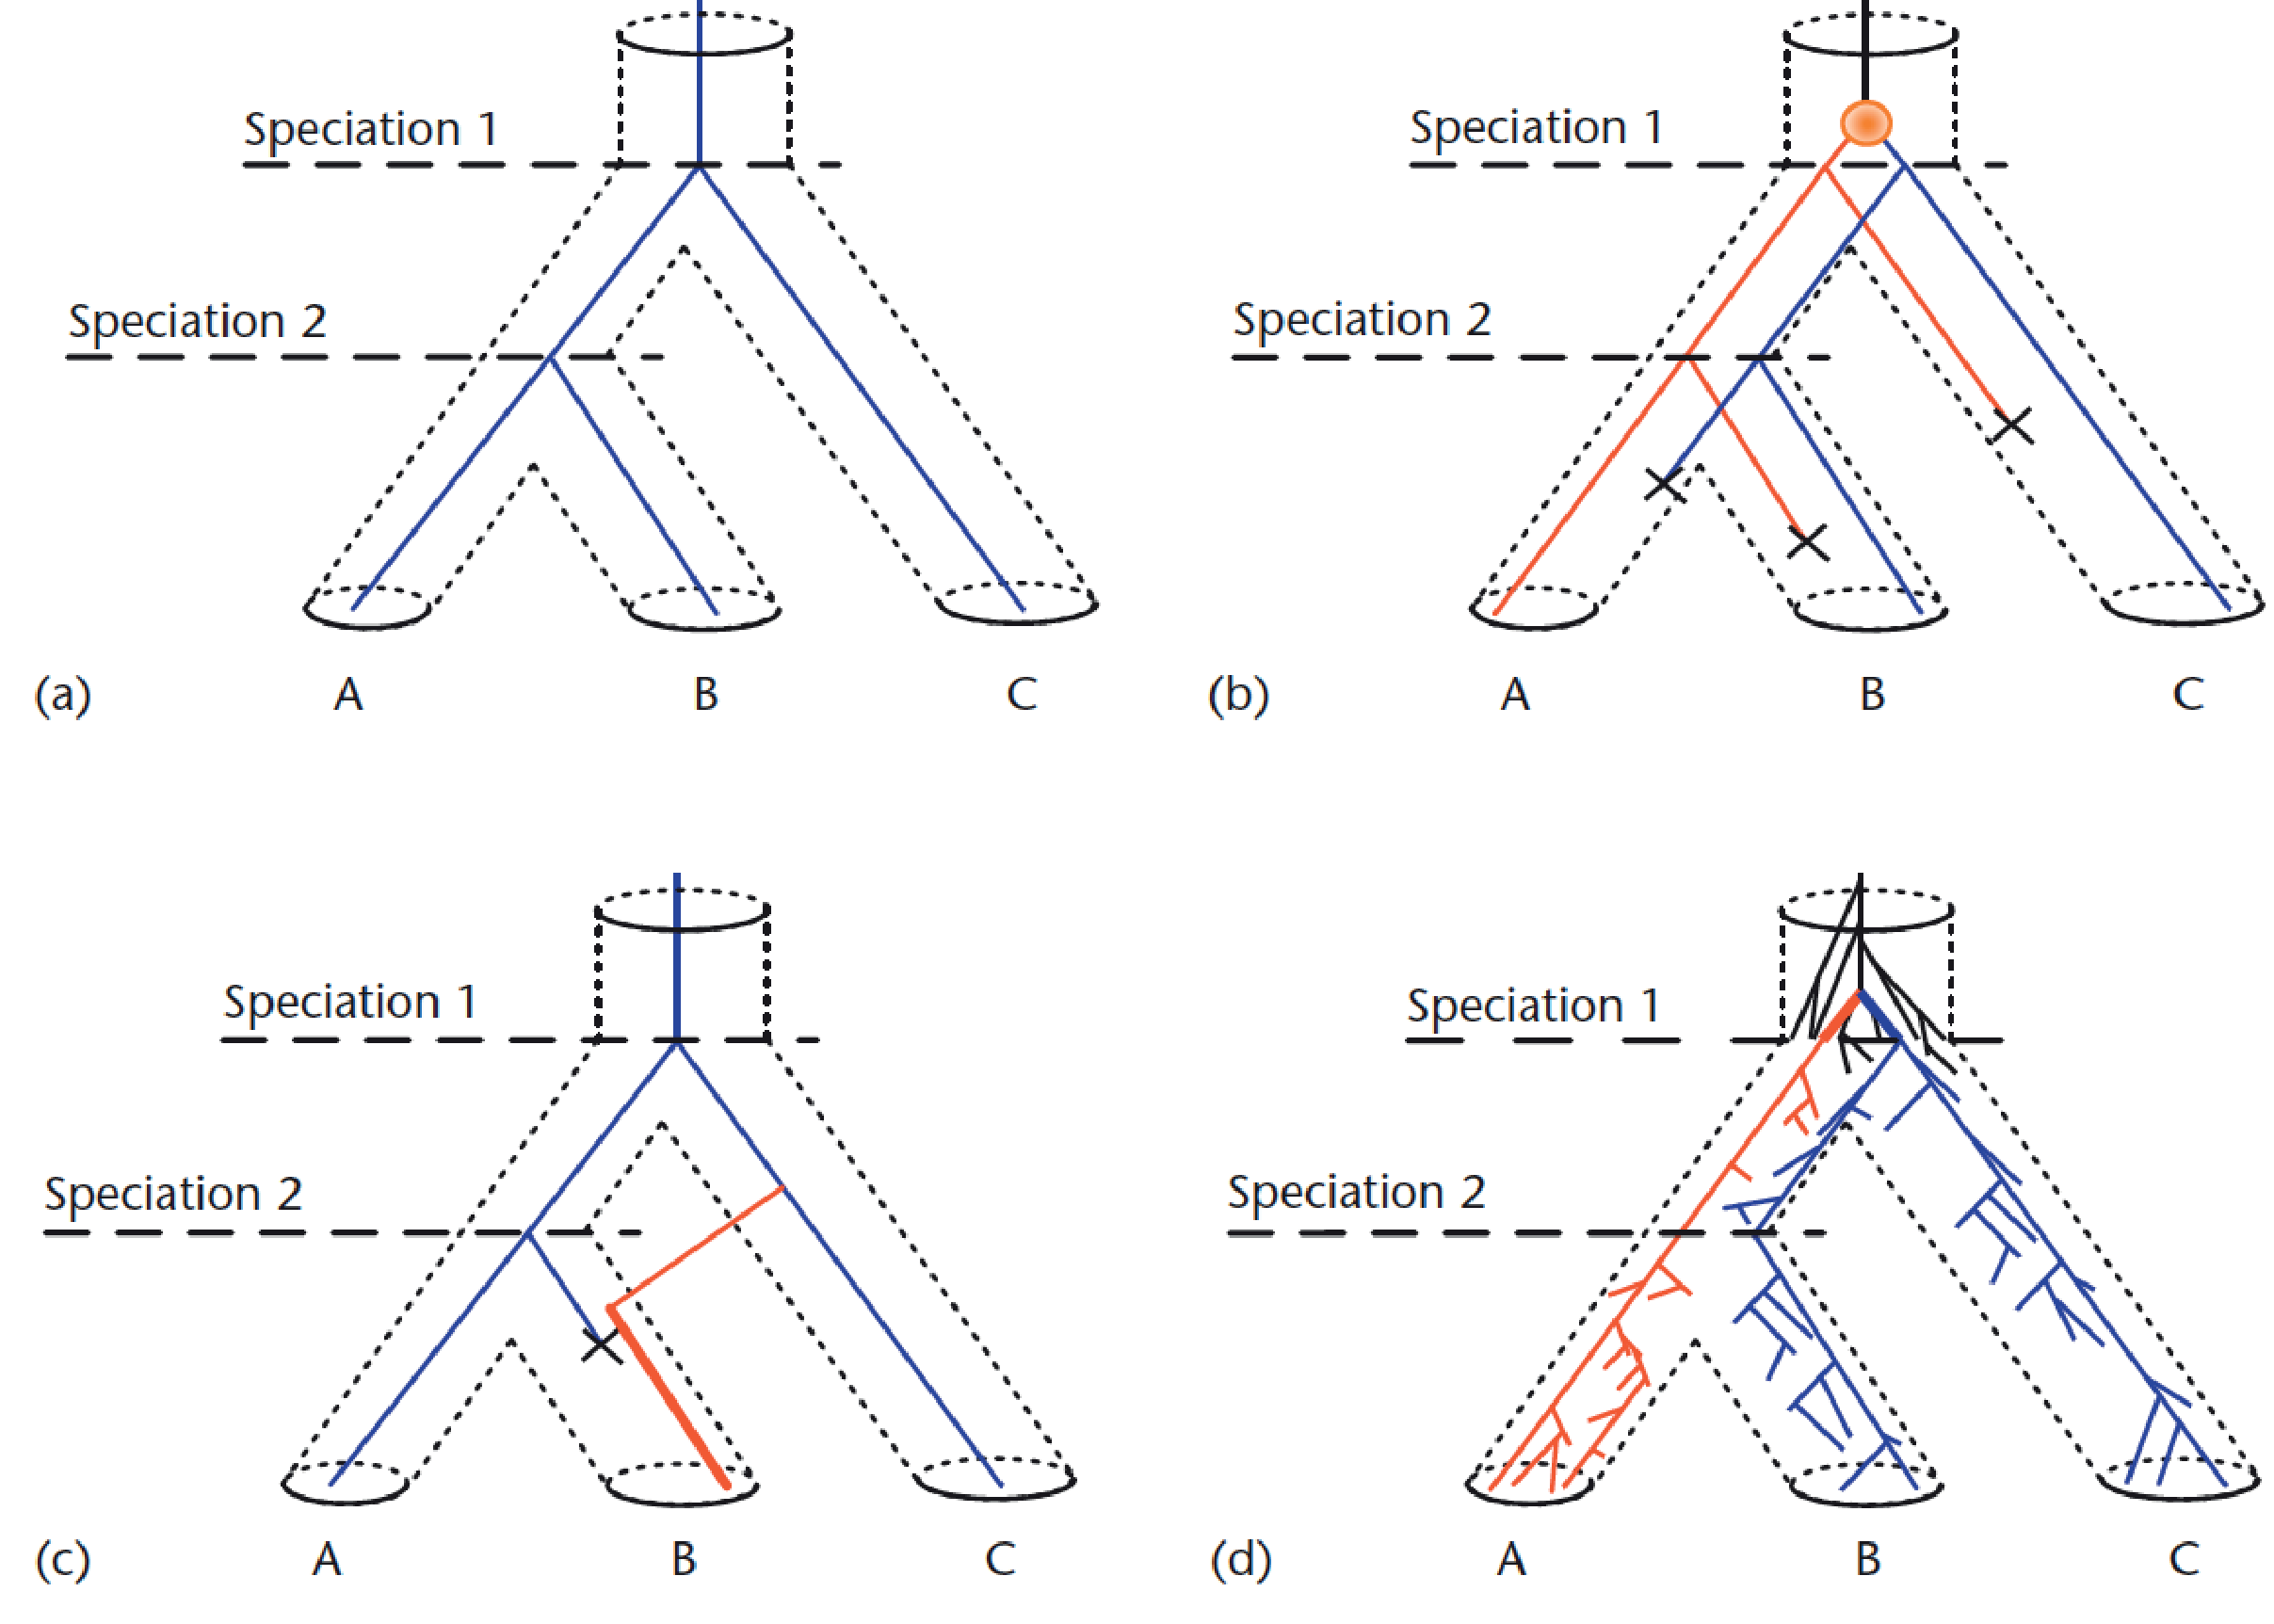
\includegraphics[width=5.8in,angle=0]{\ResourcePath figures/DupTransILS.pdf}}
\caption{\small The processes of discord. The species tree is represented as a tubular structure. Gene trees are blue and red lines running along the species trees. a) A gene tree that perfectly matches the species tree. b) The gene tree and the species tree differ because of gene duplications and losses. c)  The gene tree and the species tree differ because of gene transfer and gene loss. d)  The gene tree and the species tree differ because of incomplete lineage sorting.   [Replicated from Fig.~2 in \citet{Boussau2009}.]}
\label{fig1}
\end{figure}

Fig. \ref{fig1} suggests that for all processes the gene tree can be seen as the product of a branching process operating inside the species tree.
Indeed, all processes are modeled as some type of birth-death process running along the species tree.
For duplication/loss models, birth correspond to gene duplication events, and death to gene loss events.
Transfers can be added to the model by introducing another type of birth, with a child lineage appearing in another branch of the species tree.
Incomplete lineage sorting is also modeled with a birth-death type of model, the coalescent.
All these models can be made heterogeneous, for instance by allowing different sets of parameters for different branches of the species tree.
This is useful to model differences in rates of duplication, loss or transfer among species, or to model different effective population sizes in a species tree.
In \RevBayes~so far only models of incomplete lineage sorting have been implemented (models of duplication and loss and transfer will soon be added).
Thanks to \RevBayes~modular design, there is quite a lot of flexibility in specifying the model, for instance by associating different parameters to different branches of the species tree, or by combining the gene tree-species tree model to other types of models, for instance models of trait evolution, or models of relaxed molecular clock.


\subsection{Gene tree discordance is a problem for species tree reconstruction}
There are several approaches to species tree reconstruction: concatenation and supertree approaches, which have been used for quite some time now, and more recently methods that rely on gene tree-species tree models.\begin{enumerate}
\item Concatenation simply consists in taking all gene alignments, concatenating them into one super alignment, and then analyzing it as if it were a single gene sequence.
Its main assumption is therefore that all sites of all genes have evolved according to the same species tree.
This assumption is not correct because all the processes of discord presented above conspire to make gene trees different from the species tree.
In practice, this matters: simulation studies have found that in the presence of incomplete lineage sorting, in some particular areas of the parameter space, concatenation will often return an incorrect species tree \citep{Leache2011}.
Another example might be found in prokaryotic phylogenetics, where the quest for a tree of life has been difficult, to the point that many doubt that one could find a meaningful species tree representing vertical descent.
Recent models of gene tree evolution incorporating lateral gene transfer allow tackling this question in a more principled way.
\item Supertree approaches differ from concatenation notably by discarding sequence information once individual gene trees have been built.
Contrary to concatenation approaches that combine individual gene alignments, supertree approaches combine individual gene trees to obtain a species tree.
Most supertree methods are not based on an explicit model of the processes causing discordance between gene trees and species tree (although there are exceptions, notably modelling incomplete lineage sorting, see below).
Instead, they aim at finding a tree that would best describe the distribution of gene trees, according to some fairly arbitrary criterion.
In practice, these methods have been found to provide reasonable results in many cases, but in simulations they are usually less accurate than concatenation.
\item Methods that rely on gene tree-species tree models appear very promising as they explicitly model the processes of discord, and can be combined with \EG models of sequence evolution, models of co-evolution between gene trees, models of trait evolution... 
\end{enumerate}


\subsection{Modelling incomplete lineage sorting: the multispecies coalescent}
Incomplete lineage sorting is a population-level process.
In a species, at a given time, there are several alleles for a given locus in the genome.
These alleles have their own history, they diverged from each other at various times in the past.
This history can differ from the species history, because several alleles can persist through a speciation event, and because, without selective effects, the sorting of alleles during a speciation event is random and can result in a tree that differs from the species tree (Fig. \ref{fig1}d).
In all cases, incongruence between the gene tree and the species tree occurs when alleles persist over the course of several speciation events.
When reconstructing a gene tree, one therefore gets the history of the alleles that have been sampled (at best), not the history of the species. 

In 2003, Rannala and Yang proposed a powerful way to model the sorting of alleles along a phylogeny of several species \citep{Rannala2003a}, the multispecies coalescent (Fig. \ref{fig2}).
This model is at the origin of most model-based approaches to reconstruct gene and species trees \citep{Edwards2007,Heled2010}.
The multispecies coalescent appropriately models the evolution of a population of alleles along a species tree.
Along the species tree, it allows different branch lengths, in units of time, and also allows different effective population sizes.
Computing the probability of a gene tree given a species tree and other parameters is quite easy.
Bascially it works by cutting the gene tree into independent species-specific subtrees, computing probabilities for each of those subtrees, and combining them all at the end to get the probability of the gene tree according to the multispecies coalescent, given the current parameter values.
Cutting the gene tree into species-specific subtrees is quite easy, because we can use the dates of speciation events to identify parts of the gene trees that are before and after speciation events. 
The resulting subtrees are represented with the grey boxes in Fig. \ref{fig2}.
In this figure, each subtree corresponds to one particular population, either extant or ancestral.
Inside each subtree, given its length, the effective population size, and dates of coalescence (divergences of alleles), the coalescent model provides simple formulas for computing the probability of the gene subtree given other parameters.
Because we consider that these subtree probabilities are all independent of one another, they are then multiplied to get the gene tree probability given current parameter values.
 
Two parameters associated to branches of the species tree have a direct impact on the expected amount of gene tree-species tree incongruence:
\begin{itemize}
\item \textbf{Time between speciations.} The more a branch length increases, the more the pool of alleles is expected to change.
Alleles are therefore less likely to persist for several speciation events if the branches between these speciation events are long.
\item \textbf{Effective population size between speciations.} In populations with small effective population sizes, chance events can cause large shifts in allele frequencies, and possibly disappearance of alleles. 
In large populations, because an allele is likely carried by a large number of individuals, its disappearance is less likely, the population of alleles is more stable.
Alleles are therefore less likely to persist for several speciation events if the branches between these speciation events are characterised by small effective population sizes.
\end{itemize}
Overall, larger amounts of gene tree-species tree incongruence are expected in phylogenies characterised by short branches with large population sizes. 
A corollary of that is that larger amounts of gene tree-gene tree incongruence are expected as well. 
To measure the susceptibility of species phylogenies to generate incomplete lineage sorting, the concept of \emph{coalescent time units} has been introduced.
Coalescent time units are obtained when branch length $\lambda$, in number of generations, is divided by effective population size $N_e$.
As a consequence, in a species tree whose branches are expressed in coalescent time units, a branch length of $1~coalescent~time~unit $ means a branch length of $N_e~generations$. 
Once branch lengths on the species tree are measured in coalescent time units, it becomes easy to spot species trees that generate a lot of incongruence: those are short trees.

\begin{figure}[h!]
\centering
\fbox{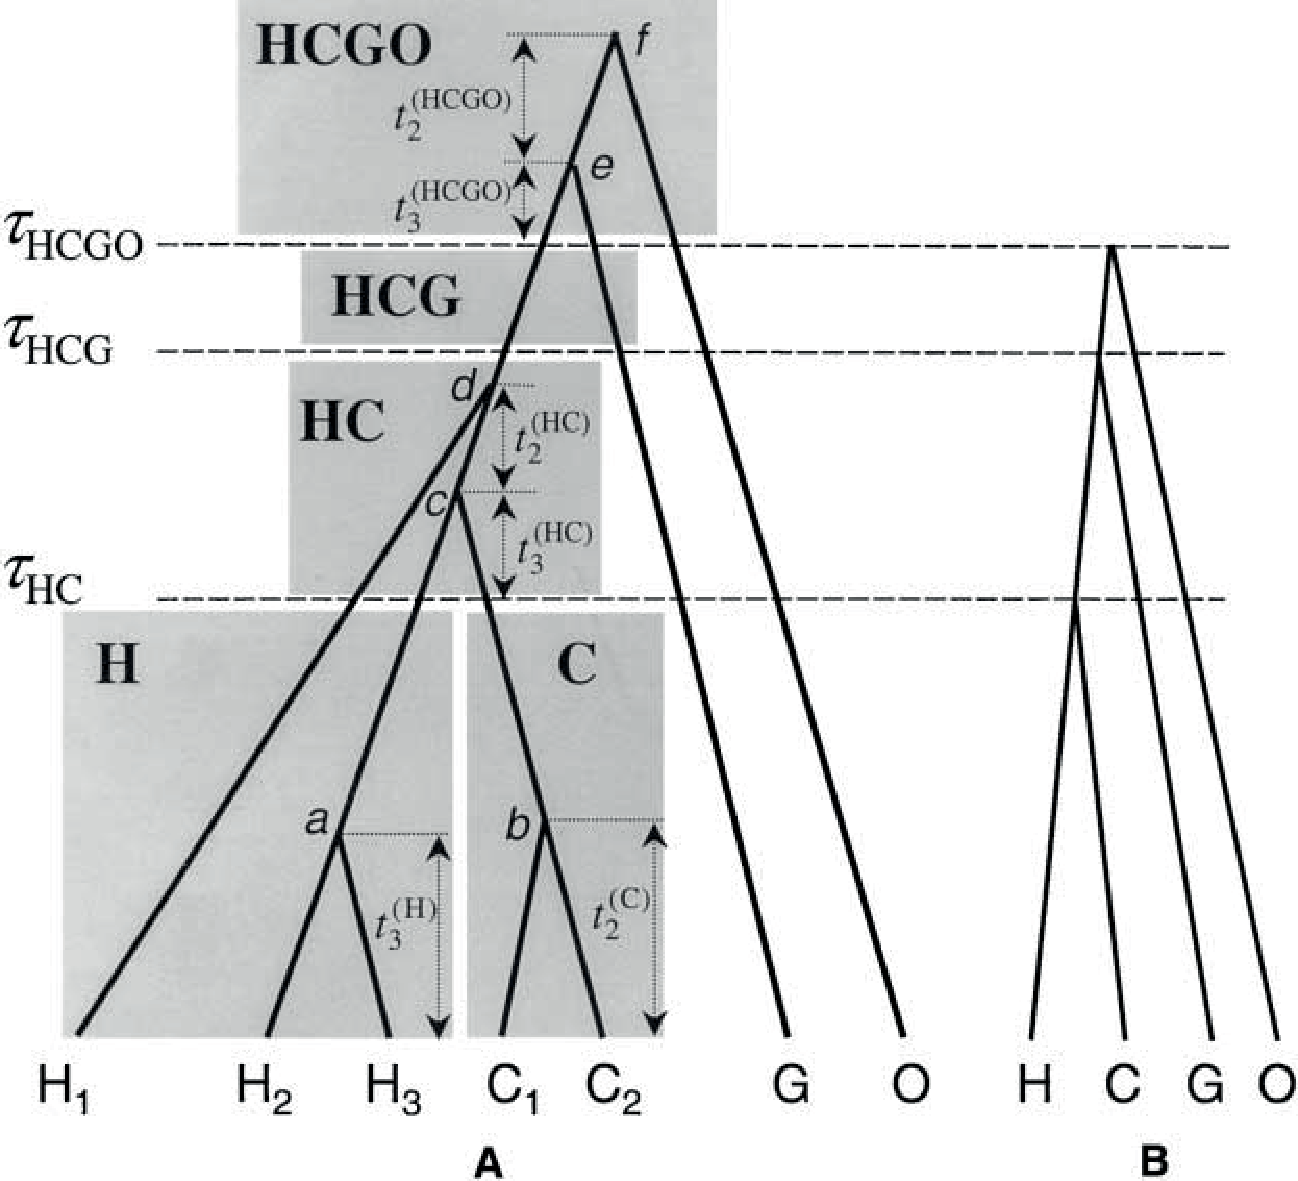
\includegraphics[width=5.8in,angle=0]{\ResourcePath figures/RannalaYang.pdf}}
\caption{\small The multispecies coalescent. A) A gene tree, including 3 human alleles, 2 Chimp alleles, one Gorilla allele, and one Orang-outan allele. $\tau$ parameters are speciation times, $t$ parameters are divergence time in the gene tree, the grey squares represent the ancestral populations, with their respeciive sizes.  B) The corresponding species tree. In this model, the speciation times define minimal boundaries for allele divergence times. [Replicated from Fig.~1 in \citet{Rannala2003a}.]}
\label{fig2}
\end{figure}

\vspace{20mm}

{\begin{framed}
\begin{center}
The exercises assume you have a working installation of RevBayes.
In this introductory tutorial, we will apply the multispecies coalescent model to 10 gene alignments from 23 mammalian species.
We will specify the multispecies coalescent, with different effective population sizes for each branch of the species tree.
We will assume that:
\begin{itemize}
\item The species tree is drawn from a constant birth-death process.
\item Along the branches of the species tree, a multispecies coalescent process generates gene trees. Different effective population sizes are assigned to each branch of the species tree.
\item Along each gene tree, gene sequences are evolved according to an HKY model with a strict clock. 
\item Here, we run an MCMC on this model, using data from 10 genes in 23 mammalian species.
\end{itemize}
Scripts are all placed in {\footnotesize \emph{$tutorials/RB\_GeneTreeSpeciesTreeSimple\_Tutorial/RB\_GeneTreeSpeciesTreeSimple\_tutorial\_files/RevBayes\_scripts/$}}. 
\end{center}
\end{framed}}
\vspace{5mm}

\begin{center}
\emph{First RevBayes exercise: loading gene alignments into RevBayes}
\end{center}
\begin{enumerate}
\item Open RevBayes
\item Let's load all 10 gene alignments.
{\tt \begin{snugshade*}
\begin{lstlisting}
locus_names = ["COIII", "FGA", "GHRmeredith", "lrpprc_169", "npas3", "sim1", "tex2", "ttr", "zfy", "zic3"]

num_loci = locus_names.size()

# read in each data matrix separately
for ( i in 1:num_loci ) {
    data[i] <- readDiscreteCharacterData("data/" + locus_names[i] + ".fasta")
}

# Now we get some useful variables from the data. We need these later on.
primate_tree = readTrees("data/primates.tree")[1]
n_species <- primate_tree.ntips()
names <- primate_tree.names()
n_branches <- 2 * n_species - 1 # number of branches in a rooted tree

# We set our move index
mi = 0
\end{lstlisting}
\end{snugshade*}}
\item We simulate a species tree topology according to a birth-death process with fixed parameter values:
{\tt \begin{snugshade*}
\begin{lstlisting}
# Specify a prior on the diversification and turnover rate
diversification ~ dnGamma(2,2)
relativeExtinction ~ dnBeta(1,1)

# Now transform the diversification and turnover rates into speciation and extinction rates
speciation := abs(diversification / (1.0 - relativeExtinction) )
extinction := speciation * relativeExtinction

# Specify a prior on the root age (our informed guess is about 75-80 mya)
root ~ dnUniform(0,1000)

# Now comes the most important trick!!!
# 
# We need to set a low root age so that in the beginning of the MCMC all lineages
# evolve in the same "root" population.
# This enables that we can quickly get good estimates of the gene-trees and then
# pull up the species tree.
root.setValue(0.001)

sampling_fraction <- 23 / 450 # we sampled 23 out of the ~ 450 primate species

# create some moves that change the stochastic variables
# Moves are sliding and scaling proposals
moves[++mi] = mvSlide(diversification,delta=1,tune=true,weight=2)
moves[++mi] = mvSlide(relativeExtinction,delta=1,tune=true,weight=2)
moves[++mi] = mvScale(diversification,lambda=1,tune=true,weight=2)
moves[++mi] = mvScale(relativeExtinction,lambda=1,tune=true,weight=2)
moves[++mi] = mvSlide(root,delta=1,tune=true,weight=0.2)
moves[++mi] = mvScale(root,lambda=1,tune=true,weight=0.2)


# construct a variable for the tree drawn from a birth-death process
psi ~ dnBDP(lambda=speciation, mu=extinction, rootAge=abs(root), rho=sampling_fraction, nTaxa=n_species, names=names )

moves[++mi] = mvNarrow(psi, weight=5.0)
moves[++mi] = mvNNI(psi, weight=1.0)
moves[++mi] = mvFNPR(psi, weight=3.0)
moves[++mi] = mvGPR(psi, weight=3.0)
moves[++mi] = mvSubtreeScale(psi, weight=3.0)
moves[++mi] = mvNodeTimeSlideUniform(psi, weight=15.0)


\end{lstlisting}
\end{snugshade*}}
\item Now that we have a species tree topology, we can have a multispecies coalescent process run along the species tree to generate gene trees.
{\tt \begin{snugshade*}
\begin{lstlisting}

# We assume independent effective population size parameters for each branch of the species tree.
for (i in 1:n_branches) {
  Ne[i] ~ dnExponential(0.1)
  moves[++mi] = mvScale(Ne[i],1,true,1.0)
}

# We could instead assume a single effective population size for the entire species tree with the following two lines:
#Ne ~ dnGamma(shape=1.0,rate=1.0)
#moves[++mi] = mvScale(Ne,1,true,1.0)

for (i in 1:num_loci) {

   # We need to read in files providing the link between gene names and species names
   taxa = readTaxonData("data/species_maps/primates_" + locus_names[i] + "_species_map.txt")

   # The gene tree from the multispecies coalescent process
   # Note that Ne is a vector of effective population sizes, 
   # allowing 1 parameter per branch of the species tree.
   geneTree[i] ~ dnCoalMultiSpeciesConst(speciesTree=psi, Ne=Ne, taxa=taxa)

   # moves on the tree
   moves[++mi] = mvNNI(geneTree[i], 5.0)
   moves[++mi] = mvNarrow(geneTree[i], 5.0)
   moves[++mi] = mvFNPR(geneTree[i], 3.0)
   moves[++mi] = mvGPR(geneTree[i], 2.0)
   moves[++mi] = mvSubtreeScale(geneTree[i], 5.0)
   moves[++mi] = mvNodeTimeSlideUniform(geneTree[i], 20.0)
   moves[++mi] = mvRootTimeSlide(geneTree[i], 1.0, true, 3.0)

}

\end{lstlisting}
\end{snugshade*}}

\item Now we have gene trees, complete with branch lengths. The aim is to simulate gene sequences along these gene trees. To do that, we need to decide how we transform time in number of generations, which are the units of the gene tree branch lengths, into time in effective number of substitutions per site. We choose to assume a strict clock, \IE a single coefficient that applies to all branches of the gene tree. However, we allow that different genes will have different values of this coefficient.
{\tt \begin{snugshade*}
\begin{lstlisting}
# We use a fixed estimate of the clock rate which is 1.00 substitution per site per million years 
# Arbitrarily, we decide that the first gene has a clock rate of 1
clockRate[1] <- 1.0

# All other genes have clock rates defined relatively to the first gene
for ( i in 2:num_loci ) { 
    relativeClockRate[i] ~ dnLognormal(0,1)
    clockRate[i] := clockRate[1] * relativeClockRate[i]
    moves[++mi] = mvScale(relativeClockRate[i],lambda=1,tune=true,weight=1)
}

\end{lstlisting}
\end{snugshade*}}

\item Now the gene tree branch lengths are in units that are appropriate for simulating gene sequences. We just need to define the substitution matrix to decide how sequences will evolve. We use a single HKY matrix that will apply to all sites, and consider that within a gene all sites evolve at the same rate of evolution.

{\tt \begin{snugshade*}
\begin{lstlisting}
for ( i in 1:num_loci ) {

    #### specify the HKY substitution model applied uniformly to all sites of a gene
    kappa[i] ~ dnLognormal(0,1)
    moves[++mi] = mvScale(kappa[i],weight=1)

    pi_prior[i] <- v(1,1,1,1) 
    pi[i] ~ dnDirichlet(pi_prior[i])
    moves[++mi] = mvSimplexElementScale(pi[i],weight=2)


    #### create a deterministic variable for the rate matrix
    Q[i] := fnHKY(kappa[i],pi[i]) 

}

\end{lstlisting}
\end{snugshade*}}


\item Now we have defined all the bricks of the model, and we need to link the model to the data.
{\tt \begin{snugshade*}
\begin{lstlisting}
for ( i in 1:num_loci ) { 
    # the sequence evolution model
    seq[i] ~ dnPhyloCTMC(tree=geneTree[i], Q=Q[i], branchRates=clockRate[i], type="DNA")

    # attach the data
    seq[i].clamp(data[i])
}
\end{lstlisting}
\end{snugshade*}}

\item Finally, we need to perform inference under the model, using the data.
{\tt \begin{snugshade*}
\begin{lstlisting}
# We get a handle on our model.
# We can use any node of our model as a handle, here we choose to use the topology.
mymodel = model(psi)

# Monitors to check the progression of the program
monitors[1] = mnScreen(printgen=100, root)
monitors[2] = mnModel(filename="output/primates_fixed_clock.log",printgen=10, separator = TAB)
monitors[3] = mnFile(filename="output/primates_fixed_clock.trees",printgen=10, separator = TAB, psi)
for ( i in 1:num_loci ) { 
    # We add a monitor for each gene tree
    monitors[i+3] = mnFile(filename="output/primates_fixed_clock_" + locus_names[i] + ".trees",printgen=10, separator = TAB, geneTree[i])
}

# Here we use a plain MCMC. You could also set nruns=2 for a replicated analysis
# or use mcmcmc with heated chains.
mymcmc = mcmc(mymodel, monitors, moves)

# This should be sufficient to obtain enough MCMC samples
mymcmc.burnin(generations=5000,tuningInterval=250)
mymcmc.run(generations=50000)
\end{lstlisting}
\end{snugshade*}}

\item Now we can perform some post-run analyses.
{\tt \begin{snugshade*}
\begin{lstlisting}
# Now, we will analyze the tree output.
# Let us start by reading in the tree trace
treetrace = readTreeTrace("output/primates_fixed_clock.trees", treetype="clock")
# and get the summary of the tree trace
treetrace.summarize()

mapTree(treetrace,"output/primates_fixed_clock.tree")


\end{lstlisting}
\end{snugshade*}}

%\end{itemize}
\end{enumerate}


\bigskip


\section{Batch Mode}

If you wish to run these exercises in batch mode, the files are provided for you. 

You can carry out these batch commands by providing the file name when you execute the \cl{rb} binary in your unix terminal (this will overwrite all of your existing run files).
\exs{\cl{\$ rb NameOfTheFile.Rev}}


\section{Things to think about}
How did the different methods perform? 
Did you expect to see these differences?
It has been shown that the concatenation approach could be inconsistent under some conditions of population size and of divergence times \citep{Degnan2006}. 
Do you find that concatenation performs worse that its competitors?
Which models seem to "mix" better?
In particular, does the full multispecies coalescent mix well?
Why can we expect this model in particular would have difficulties mixing?


\bigskip
\section{Useful Links}

\begin{itemize}
\item RevBayes: \href{https://github.com/revbayes/code}{https://github.com/revbayes/code} \\ \vspace{-7mm}
\item Tree Thinkers: \href{http://treethinkers.org/}{http://treethinkers.org} \\ \vspace{-7mm}
\item NJplot, a lightweight tree plotting program: \href{http://doua.prabi.fr/software/njplot}{http://doua.prabi.fr/software/njplot} \\ \vspace{-7mm}
\item Seaview, a program to handle alignments and trees: \href{http://doua.prabi.fr/software/seaview}{http://doua.prabi.fr/software/seaview} \\ \vspace{-7mm}

\end{itemize}

Questions about this tutorial can be directed to: \\\vspace{-10mm}
\begin{itemize}
\item Bastien Boussau (email: \href{mailto:boussau@gmail.com}{boussau@gmail.com}) \\\vspace{-8mm}
\item Sebastian H\"{o}hna (email: \href{mailto:sebastian.hoehna@gmail.com}{sebastian.hoehna@gmail.com})
\end{itemize}


\bibliographystyle{mbe}
\bibliography{\ResourcePath refs}

